DIAL (DIscovery And Launch) es el antiguo protocolo de comunicación que usaba Chromecast, desarrollado con Netflix y Youtube.
Se basa en Universal Plug and Play (UPnP), Simple Service Discovery Protocol (SSDP) y protocolos HTTP.
SSDP es un protocolo que sirve para la búsqueda de dispositivos UPnP en una red. Utiliza UDP en unicast o multicast en el puerto 1900 para anunciar los servicios de un dispositivo. Si el receptor ofrece el servicio deseado devuelve el mensaje '200 OK' con HTTP.


\begin{figure}[H]
	\centering
	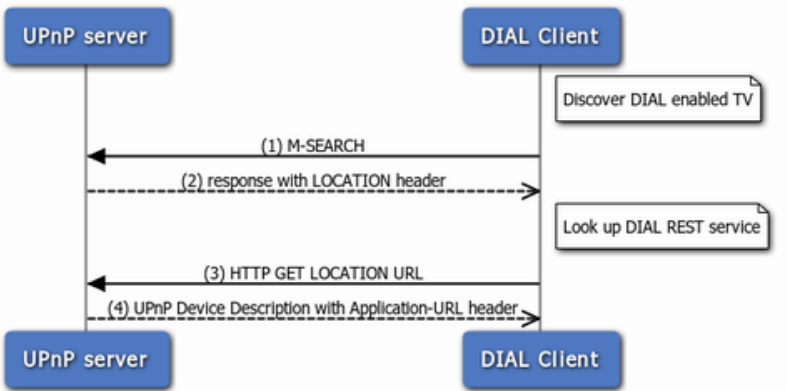
\includegraphics[scale=0.32]{./Imagenes/dial.png}
	\caption{Funcionamiento general DIAL}
	\label{fig:DIAL}
\end{figure}


DIAL permite a dispositivos en segundo plano, como tablets o móviles, enviar contenido a dispositivos en primer plano, por ejemplo televisiones.
Los dispositivos en segundo plano almacenarán el cliente, los de primer plano ejecutarán el servidor.
Para evitar conflictos con los nombres de aplicaciones permitidas DIAL tiene un registro con las aplicaciones que soporta. En el caso de que la aplicación deseada no esté en esa lista puede que tenga un prefijo que esté registrado, para así ofrecer mayor flexibilidad.

El protocolo DIAL tiene dos componentes, DIAL Service Discovery y DIAL REST Service.
El primero busca el dispositivo en primer plano dentro de una red local y permite establecer conexión.
El segundo permite al cliente mandar contenido, hacer consultas como subir o bajar volumen, etc. al servidor.
El servidor puede procesar mensajes de hasta 4KB.

\begin{figure}[H]
	\centering
	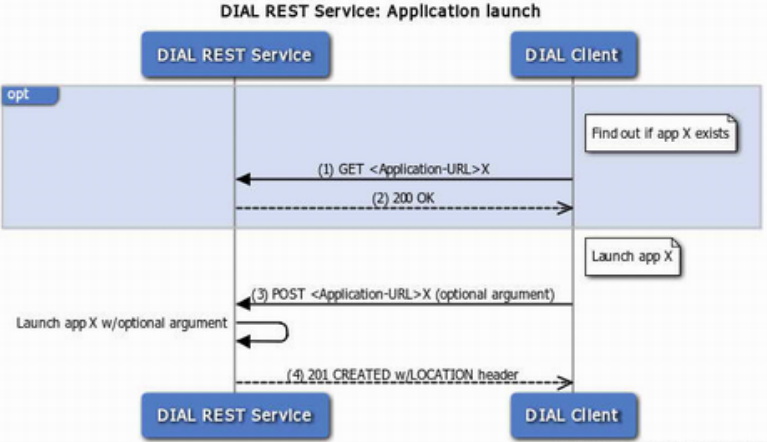
\includegraphics[scale=0.5]{./Imagenes/dialrest.png}
	\caption{Funcionamiento DIAL REST service}
	\label{fig:DIAL}
\end{figure}


Las respuestas específicas y otros detalles como manejo de excepciones se pueden encontrar en \cite{dial}
